\documentclass[10pt]{article}
\usepackage[letterpaper,margin=0.55in]{geometry}
\usepackage[T1]{fontenc}
\usepackage{lmodern,microtype}
\usepackage{amsmath,amssymb,mathtools}
\usepackage{booktabs,tabularx,array}
\newcolumntype{Y}{>{\raggedright\arraybackslash}X}
\usepackage[most]{tcolorbox}
\usepackage{tikz}
\usetikzlibrary{arrows.meta,positioning,calc}
\usepackage{enumitem}
\usepackage{xcolor}
\usepackage{fancyhdr}
\usepackage{hyperref}
\definecolor{navy}{HTML}{15324A}
\definecolor{teal}{HTML}{167D7F}
\definecolor{sky}{HTML}{DCEFF2}
\definecolor{gold}{HTML}{D99A2B}
\definecolor{amber}{HTML}{FFF3D6}
\definecolor{brick}{HTML}{A83F39}
\definecolor{rose}{HTML}{F7E4E2}
\definecolor{ink}{HTML}{20262D}
\definecolor{mist}{HTML}{F4F7F9}
\definecolor{green}{HTML}{2C7A4B}
\definecolor{lightgreen}{HTML}{E7F3EB}
\color{ink}
\hypersetup{colorlinks=true,linkcolor=navy,urlcolor=brick,pdftitle={Comparative Metric Learning for Robust Pose Retrieval - Brief Proposal},pdfauthor={Giacomo Cappelletto}}
\pagestyle{fancy}\fancyhf{}\fancyhead[L]{\small\textcolor{navy}{Comparative pose metric learning}}\fancyhead[R]{\small\textcolor{navy}{Brief proposal}}\fancyfoot[C]{\small\thepage}\renewcommand{\headrulewidth}{0.3pt}
\setlength{\parindent}{0pt}\setlength{\parskip}{3pt}
\newtcolorbox{pitchbox}[1][]{enhanced,colback=sky,colframe=teal,boxrule=.8pt,arc=1.5mm,left=2mm,right=2mm,top=1.5mm,bottom=1.5mm,#1}
\newtcolorbox{warnbox}[1][]{enhanced,colback=rose,colframe=brick,boxrule=.8pt,arc=1.5mm,left=2mm,right=2mm,top=1.5mm,bottom=1.5mm,#1}
\newtcolorbox{meetbox}[1][]{enhanced,colback=amber,colframe=gold,boxrule=.8pt,arc=1.5mm,left=2mm,right=2mm,top=1.5mm,bottom=1.5mm,#1}
\newtcolorbox{implbox}[1][]{enhanced,colback=lightgreen,colframe=green,boxrule=.8pt,arc=1.5mm,left=2mm,right=2mm,top=1.5mm,bottom=1.5mm,#1}
\tikzset{block/.style={rounded corners=1.5mm,draw=navy,thick,fill=mist,minimum height=8mm,align=center,inner sep=3pt},data/.style={rounded corners=1.5mm,draw=teal,thick,fill=sky,minimum height=8mm,align=center,inner sep=3pt},loss/.style={rounded corners=1.5mm,draw=brick,thick,fill=rose,minimum height=8mm,align=center,inner sep=3pt},arrow/.style={-{Latex[length=2mm]},thick,draw=navy!70}}
\newcommand{\sg}{\operatorname{sg}}
\newcommand{\ind}{\mathbb{1}}
\begin{document}

{\sffamily\bfseries\color{navy}\fontsize{19}{22}\selectfont Comparative Metric Learning for\\ Robust Pose-Sequence Retrieval}\par
{\large Updated research-proposal brief}\hfill{\small July 31, 2026}
\vspace{2mm}\hrule height 1pt\vspace{3mm}

\begin{pitchbox}[title=\textbf{60-second pitch}]
I will begin with the accepted pipeline: a fixed pretrained motion encoder, a clean reference gallery, and controlled pose corruptions to test whether contextual neighborhoods preserve retrieval better than standard objectives. Once that result is stable, I will keep the encoder and evaluator fixed and map the metric-learning losses evaluated in the 2023 contextual paper into the pose domain. A final screened extension will test selected post-2023 image and pose objectives. The outputs are retrieval and degradation curves plus an applicability map covering performance, robustness, compute, and implementation changes.
\end{pitchbox}

\begin{warnbox}[title=\textbf{Scientific boundary}]
The foundation paper establishes reduced overfitting and label-noise robustness for \emph{image retrieval}; it does not prove pose-input robustness. Its tables also mix controlled loss re-runs with copied results from architecture-changing methods. The primary pose comparison includes the former, not every row indiscriminately.
\end{warnbox}

\textbf{Method in one picture}
\begin{center}
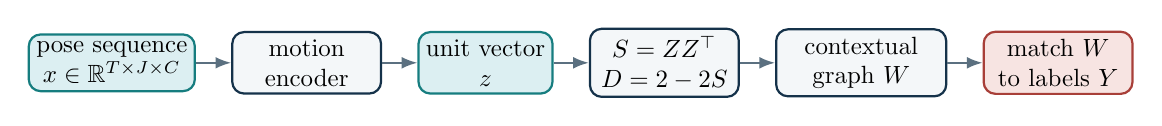
\begin{tikzpicture}[node distance=5mm,scale=.9,transform shape]
\node[data,minimum width=22mm] (x) {pose sequence\\$x\in\mathbb R^{T\times J\times C}$};
\node[block,right=of x,minimum width=21mm] (e) {motion\\encoder};
\node[data,right=of e,minimum width=18mm] (z) {unit vector\\$z$};
\node[block,right=of z,minimum width=21mm] (s) {$S=ZZ^\top$\\$D=2-2S$};
\node[block,right=of s,minimum width=24mm] (n) {contextual\\graph $W$};
\node[loss,right=of n,minimum width=21mm] (l) {match $W$\\to labels $Y$};
\draw[arrow](x)--(e);\draw[arrow](e)--(z);\draw[arrow](z)--(s);\draw[arrow](s)--(n);\draw[arrow](n)--(l);
\end{tikzpicture}
\end{center}

\textbf{Five equations to narrate}
\begin{align*}
D(i,j)&=\lVert z_i-z_j\rVert_2^2=2-2s_{ij}.\\[-2pt]
N_{ij}&=\theta\!\left(-D(i,j)+\sg(D(i,p_k))+\epsilon\right),
\quad \frac{\partial\theta}{\partial x}=\alpha.\\[-2pt]
W_1(i,j)&=\frac{N_{ij}}{2}\left[\frac{M_+(i,j)}{\sg\sum_pN_{ip}}+\frac{M_-(i,j)}{\sg\sum_p(1-N_{ip})}\right].\\[-2pt]
W_2&=\frac{RW_1}{R\mathbf 1},\qquad W=\tfrac12(W_2+W_2^\top),\quad R=N_{k/2}\odot N_{k/2}^\top.\\[-2pt]
\mathcal L&=\lambda\,\frac{1}{n^2}\sum_{i\ne j}(y_{ij}-w_{ij})^2+(1-\lambda)\mathcal L_{\rm contrast}+\gamma\mathcal L_{\rm reg}.
\end{align*}

\begin{meetbox}[title=\textbf{The key theoretical statement}]
For a balanced batch with exactly $k$ samples per class, $n>2k$, and $\epsilon=0$, zero contextual loss occurs exactly when every positive ranks ahead of every negative within the batch. This is why $k$ is tied to samples per class rather than treated as an unrelated top-$k$ hyperparameter.
\end{meetbox}

\newpage
{\sffamily\bfseries\color{navy}\Large Staged comparison and discussion answers}\vspace{2mm}\hrule\vspace{3mm}

\textbf{Controlled experiment}\par\vspace{1mm}
{\small
\renewcommand{\arraystretch}{1.06}
\begin{tabularx}{\textwidth}{>{\bfseries\raggedright\arraybackslash}p{0.19\textwidth}Y}
\toprule
Component & Decision \\
\midrule
Dataset & NTU RGB+D 120; official cross-subject and cross-setup protocols. \\
Encoder & Pretrained MotionBERT sequence encoder; normalized projection output. \\
Retrieval & Disjoint query/gallery manifest; noisy queries against a fixed clean gallery. \\
Stage I & Cross-entropy embedding, SupCon, triplet/Multi-Similarity, contextual, contextual+contrastive, and corruption-aware SupCon. \\
Stage II & Core 2023 reruns: contrastive, mined triplet, Multi-Similarity $\pm$ miner, Proxy Anchor/NCA, ROADMAP, and contextual. Appendix tier: NT-Xent, Fast-/Smooth-AP, then supplemental AP and reported proxy losses. \\
Stage III & Core recent screen: SGSL, mean-field DML, and PFML. Method-faithful pilots: SimPLE and 2026 NC-Init+PI. Pose controls: continuous-label triplet, MaskCLR, class-aware contrast, and USDRL. \\
Stage IV & Whole-system transfer, reported separately: IBC, S2SD, Metrix, and HIST first; then DRML, DIML, DiVA, MHGL, and AVSL if resources permit. \\
Corruptions & Gaussian joint jitter; random joint/limb masking; frame dropout; 3D yaw rotation; pose-estimator shift when available. \\
Metrics & Recall@1/5/10, mAP, retention $M(c)/M(0)$, and degradation $\Delta(c)=M(0)-M(c)$. \\
Fairness & Strict track fixes backbone, embedding geometry, sampler, split, evaluator, tuning budget, augmentations, and seeds. Method-faithful variants are reported separately. \\
\bottomrule
\end{tabularx}}

\begin{implbox}[title=\textbf{Lowest-risk implementation sequence}]
\begin{enumerate}[leftmargin=*,itemsep=1pt,topsep=1pt]
\item Freeze MotionBERT; validate splits, cosine retrieval, metrics, and deterministic corruptions.
\item Train only small projection heads with SupCon, contextual, and hybrid losses.
\item Complete representative pairwise, proxy, and AP/rank families before appendix-grade losses.
\item Profile time/memory and fine-tune the encoder only after the loss matrix is stable.
\item Select two or three recent methods with distinct mechanisms and reliable implementations.
\item Add pose-specific controls; broaden the dataset only after the NTU study is complete.
\end{enumerate}
\end{implbox}

\textbf{Likely questions and precise answers}\par\vspace{1mm}
{\small
\renewcommand{\arraystretch}{1.05}
\begin{tabularx}{\textwidth}{>{\bfseries\raggedright\arraybackslash}p{0.29\textwidth}Y}
\toprule
Question & Answer \\
\midrule
What changed after the meeting? & The original contextual robustness study remains Stage I. The new contribution is a controlled transfer map of older and newer optimization families with the same pose encoder. \\
Does ``all 2023 algorithms'' mean every table row? & The loss reruns form the causal same-encoder comparison. Copied architecture/framework rows remain a later whole-system transfer tier, with every deviation logged. \\
Why retrieval rather than classification? & Classification can remain acceptable while the ordering of the embedding space deteriorates. Retrieval measures whether examples remain inspectable and useful for one-shot decisions. \\
How is applicability measured? & Clean retrieval, degradation under each corruption, time/memory, seed and tuning stability, batch requirements, and whether the method needs changes beyond the loss. \\
Why two fairness tracks? & Some methods add proxies, queues, learned scorers, masking, or decoders. A strict loss track isolates the objective; a method-faithful track measures practical transfer while logging every deviation. \\
What would a null or reversed result mean? & It would show that robustness comes mainly from the encoder/corruption exposure, or that image-domain objective rankings do not transfer to temporal pose embeddings. \\
\bottomrule
\end{tabularx}}

\begin{warnbox}[title=\textbf{Do not claim}]
Do not claim that action-class retrieval measures movement quality, that label-noise robustness implies pose-noise robustness, or that copied state-of-the-art rows are controlled baselines. The contribution is a staged, retrieval-first transfer study of optimization methods.
\end{warnbox}

\textbf{Closing sentence.} \emph{The project begins with one falsifiable robustness question, then asks which metric-learning principles genuinely survive the move from images to pose sequences.}

\end{document}
